\documentclass[10pt,conference]{IEEEtran}
\usepackage[utf8]{inputenc}
\usepackage[T1]{fontenc}
\usepackage{graphicx}
\usepackage{xurl}
\usepackage{hyperref}
\usepackage{enumitem}
\usepackage{cite}
\usepackage{tikz}
\usepackage{pgfplots}
\usepackage{tabularx}
\usetikzlibrary{positioning,arrows.meta,calc,fit}
\pgfplotsset{compat=1.17}

\hypersetup{colorlinks=true, linkcolor=black, citecolor=black, urlcolor=blue}
\setlist[enumerate]{topsep=2pt,itemsep=1pt,parsep=0pt,leftmargin=*}
\setlist[itemize]{topsep=2pt,itemsep=1pt,parsep=0pt,leftmargin=*}

\newcommand{\code}[1]{\texttt{#1}}
\newcommand{\mail}[1]{\href{mailto:#1}{#1}}
\renewcommand{\arraystretch}{1.15}
\newcolumntype{Y}{>{\raggedright\arraybackslash}X}

\definecolor{cbuilt}{RGB}{190,225,190}
\definecolor{cnot}{RGB}{235,235,235}
\definecolor{cdone}{RGB}{60,120,170}
\definecolor{cpr}{RGB}{150,190,225}

\title{Can a Small Planner Fix Kubernetes Incidents? Retrieval, Tools and Fine-Tuning on
AIOpsLab: Final Report}

\author{%
\begin{tabular}{@{}c@{\hspace{0.9em}}c@{\hspace{0.9em}}c@{\hspace{0.9em}}c@{}}
\normalsize Abhinav Borah & \normalsize Dhawal Pawanarkar & \normalsize Gargi Saini & \normalsize Vivek Dhayal M K\\
\footnotesize\mail{abhinav.borah@students.iiit.ac.in} &
\footnotesize\mail{dhawal.pawanarkar@students.iiit.ac.in} &
\footnotesize\mail{gargi.saini@students.iiit.ac.in} &
\footnotesize\mail{vivekdhayal.mk@students.iiit.ac.in}
\end{tabular}}

\begin{document}
\maketitle

\noindent{\bfseries\textit{Abstract.}\quad We set out to test a small fine-tuned validity gate
that picks working Kubernetes fix commands among a planner's candidates. A headroom check on
execution-labelled candidates failed twice (0, then 1 recoverable problem of 16, against 5
needed), so the gate was not trained. We report instead what the evidence supports, on 16
AIOpsLab mitigation problems at two seeds: a Qwen3.5-4B planner with retrieval and read-only tools
recovers 6 problems at both seeds; giving it an error bundle in place of interactive telemetry
tools recovers 9; retrieval matters (2 of 16 without it); and a LoRA fine-tune of the planner on
its own working commands is falsified against the untuned planner (0 wins, 2 losses). The
largest failure class is fixes the allow-list refuses, more often than wrong diagnoses.}

\medskip
\noindent Course CL3410, Language Models and Agents, Monsoon 2026. Final submission:
2026-11-15.

\vspace{2pt}
\noindent\textbf{Code:} {\small\url{https://github.com/abhinavborah/k8s-RemValGate}}

\section{Introduction}

An agent that repairs a microservice incident has to do two things right: find the fault, and
apply a command that removes it without breaking anything else. We study both steps on the
mitigation problems of AIOpsLab~\cite{aiopslab}, where a fix counts only if the injected fault is
gone after the command runs.

Our original question was whether a small gate, fine-tuned with LoRA, selects working candidate
commands better than the planner's own ranking. That question needs candidates to choose between:
problems where the planner's first choice fails and another candidate works. We measured that
count before training (Section~\ref{sec:headroom}), it was too small, and the gate was not
trained. The capabilities the project still tests, and why:

\begin{itemize}
\item \textbf{Retrieval:} grounds the planner in earlier fixes of the same fault type. Ablated with
no retrieval, dense retrieval, and dense retrieval with a reranker.
\item \textbf{Tool calling:} the planner reads cluster state through read-only tools. Ablated in a
2 by 2 of telemetry tools against a fixed error bundle.
\item \textbf{Fine-tuning:} the planner is LoRA-tuned on its own commands that worked, and compared
with the untuned planner on a rule fixed before the result.
\end{itemize}

\noindent Contributions are measurements, not systems: a protocol with two seeds, interleaved
arms and a logged evaluation set; the capability ablations; a pre-specified, falsified fine-tuning
claim; and a failure analysis that locates the bottleneck.

\section{System}

% System of the final report: the planner acts on its own command, and the allow-list is the
% only check before execution. No gate is in the loop (#46, #49 closed as not planned).
\begin{figure*}[!t]
\centering
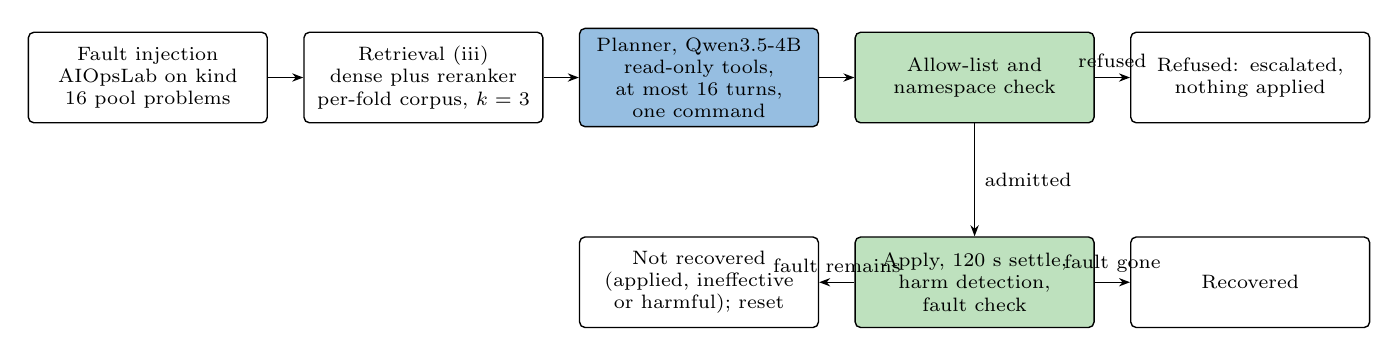
\begin{tikzpicture}[
  font=\scriptsize,
  box/.style={draw,rounded corners=2pt,minimum width=2.9cm,minimum height=1.15cm,align=center,text width=2.8cm,line width=0.5pt,fill=white},
  model/.style={box,fill=cpr},
  check/.style={box,fill=cbuilt},
  arr/.style={-{Stealth[length=4pt]},line width=0.5pt}]
\node[box]   (F)  at (0,0)     {Fault injection\\AIOpsLab on kind\\16 pool problems};
\node[box]   (R)  at (3.5,0)   {Retrieval (iii)\\dense plus reranker\\per-fold corpus, $k=3$};
\node[model] (P)  at (7,0)     {Planner, Qwen3.5-4B\\read-only tools,\\at most 16 turns,\\one command};
\node[check] (A)  at (10.5,0)  {Allow-list and\\namespace check};
\node[box]   (E)  at (14,0)    {Refused: escalated,\\nothing applied};
\node[check] (S)  at (10.5,-2.6) {Apply, 120 s settle,\\harm detection,\\fault check};
\node[box]   (OK) at (14,-2.6) {Recovered};
\node[box]   (X)  at (7,-2.6)  {Not recovered\\(applied, ineffective\\or harmful); reset};
\draw[arr] (F) to (R);
\draw[arr] (R) to (P);
\draw[arr] (P) to (A);
\draw[arr] (A) to node[above] {refused} (E);
\draw[arr] (A) to node[right] {admitted} (S);
\draw[arr] (S) to node[above] {fault gone} (OK);
\draw[arr] (S) to node[above] {fault remains} (X);
\end{tikzpicture}
\caption{The system as evaluated. The planner diagnoses with read-only tools and gives one command;
the allow-list is the only check before it runs. The validity gate of the original design was not
trained (Section~\ref{sec:headroom}).}
\label{fig:system}
\end{figure*}


Figure~\ref{fig:system} shows the system as evaluated. AIOpsLab~\cite{aiopslab} injects a fault
into the Social Network or Hotel Reservation application on a two-node kind cluster. The planner
(Qwen3.5-4B, GGUF Q8\_0, context 32768, thinking on) retrieves three past fixes with configuration
(iii), dense retrieval with a cross-encoder reranker over a per-fold corpus, then runs a loop of
at most 16 turns: each turn it calls one read-only tool (\code{kubectl get} or \code{describe},
logs, metrics, traces) or gives its diagnosis and one command.

The command must pass a deterministic allow-list (binary, namespace sandbox, verb, resource and
flags) before it runs. An admitted command is applied, the cluster settles for 120~s, harm is
detected by pod-status differencing, and the fault check decides whether the service recovered.
Kubernetes objects are snapshotted and restored on failure. The model makes a choice in one place
only, the planner's loop; retrieval, the allow-list, execution, reset and the outcome classes run
the same procedure whatever the fault.

\section{Data and evaluation protocol}

\textbf{Problems.} The pool has 16 mitigation problems of 5 fault types: TargetPortMisconfig (6),
ScalePod (3), AssignNonExistentNode (3), RevokeAuth (2) and UserUnregistered (2), split into 4
folds so that a problem never retrieves or trains on its own record. Three development problems
are used for dry runs, a 3-problem confirmation slice was sealed at the start and opened once at
the end, and 5 singleton fault types test unseen faults.

\textbf{Touch log.} Every use of an evaluation problem, a run or a read of its labels, appends an
entry to a committed touch log before it happens, and the run is refused otherwise.

\textbf{Protocol.} After three defects shared by every planner run were found (a wrong fault-type
description, tool advice that discouraged telemetry, and a retrieval query that changed between
runs), all planner results were run again from one commit (\#165). Every compared system runs at
seeds 1000 and 1001, interleaved by problem, with the model build recorded in each manifest. A
problem counts as recovered only if it recovers at both seeds.

\section{Baselines}

Table~\ref{tab:baselines} lists the baselines on the pool.

\begin{table}[!t]
\caption{Baselines on the 16 pool problems. Recovered problems; for the planner arms, at both
seeds. Qwen3.5-4B, revision 851bf6e, GGUF Q8\_0.}
\label{tab:baselines}
\centering\footnotesize
\begin{tabularx}{\columnwidth}{@{}lYr@{}}
\hline
Baseline & What & Recovered \\
\hline
1 & fault-type rule, no model\textsuperscript{a} & 8 \\
2 & top retrieved fix, no model\textsuperscript{a} & 8 \\
3a & untuned planner, no retrieval & 2 \\
3b & untuned planner, dense retrieval & 6 \\
3c & untuned planner, retrieval (iii) & 6 \\
5 & fine-tuned ranking of 3c's candidates & 7.0 \\
6 & prompted judge over 3c's candidates & 8 \\
7 & 3c told to escalate when unsure & 3 \\
\hline
\multicolumn{3}{@{}p{\columnwidth}@{}}{\scriptsize \textsuperscript{a}One run per problem, 2026-11-08 and 09,
before the rerun. Planner arms: \#165 step 1, LM Studio, 2026-11-13. Baselines 5 and 6 rank the
candidates of the step 2 labels at seed 0 (2026-11-14 and 15).}\\
\end{tabularx}
\end{table}

\section{The headroom check and why the gate was not trained}
\label{sec:headroom}

A gate can only win where the planner's top pick fails and another candidate works. Before any
gate or planner training, gate G3 labelled all $K=8$ candidates of the untuned planner by
execution and required at least 5 such recoverable problems, the smallest gain the paired test can
show at $n=16$ (5 wins with no loss, or 7 with one). The first labels gave 0 recoverable problems
and the labels after the rerun gave 1. The check failed both times, so no selector over these
candidates can gain more than one problem, and the gate was not trained. The planner acts on its
own command, and the allow-list is the only check before it runs. Baselines 5 and 6, which rerank
the same candidates, are bounded the same way: 7.0 and 8 of 16.

\section{Results}

\subsection{Fine-tuning the planner (pre-specified, exploratory)}

The decision to fine-tune the planner came after the failed headroom check, so the comparison is
exploratory. Its rule was fixed on the issue tracker before the result existed: the claim
\emph{3cft recovers more pool problems than 3c and loses at most one problem 3c recovers} is
supported only with at least 5 wins and no loss, or at least 7 wins and one loss, at both seeds;
two or more losses falsify it.

Each fold's adapter (LoRA rank 16, alpha 32, 3 epochs) was trained on the working commands of the
12 problems outside the fold, 6 to 9 records per fold, and merged into the base model. Both arms
were served by the same llama.cpp build on one A100 host and run interleaved (\#165 step 3,
2026-11-14).

\begin{table}[!t]
\caption{Fine-tuned (3cft) against untuned (3c) planner, recovered problems of 16. \#165 step 3,
llama.cpp \code{61dbf49}, 2026-11-14.}
\label{tab:finetune}
\centering\footnotesize
\begin{tabularx}{\columnwidth}{@{}Yrrrrr@{}}
\hline
 & 3c & 3cft & wins & losses & mid-p \\
\hline
both seeds (claim) & 7 & 5 & 0 & 2 & 0.25 \\
seed 1000 & 7 & 7 & 1 & 1 & 0.75 \\
seed 1001 & 10 & 8 & 1 & 3 & 0.375 \\
\hline
\end{tabularx}
\end{table}

Table~\ref{tab:finetune} gives the result: 0 wins and 2 losses at both seeds, with a Bonett-Price
95 percent interval for the difference of $[-0.32, 0.10]$. \textbf{The claim is falsified.} Both
losses are one seed's failure on a problem the planner can solve: a turn cap with no diagnosis,
and a command the allow-list refused. Labelled by execution at seed 0, the fine-tuned planner's
top pick solves 8 problems against 7, with 55 of 120 working candidates against 53 of 128, one
mixed problem and no recoverable one. Training on its own successes adds no knowledge of the fixes
it never produced: no fold holds a working MongoDB command.

\subsection{Capability ablations (descriptive)}

% Recovered pool problems per arm, rerun step 1 (commit ffc2af6, 2026-11-13), from
% docs/ablations.md and, for arm 7, docs/baselines_pool.md. "Both seeds" counts a problem only when it recovered at seeds 1000 and 1001.
\begin{figure}[!t]
\centering
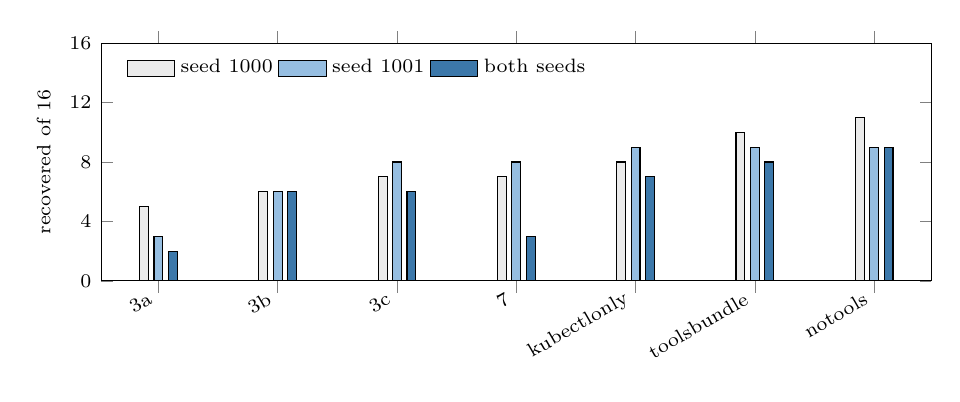
\begin{tikzpicture}
\begin{axis}[
  ybar, bar width=3.2pt, width=\columnwidth, height=4.6cm,
  ymin=0, ymax=16, ytick={0,4,8,12,16}, ylabel={recovered of 16},
  symbolic x coords={3a,3b,3c,7,kubectlonly,toolsbundle,notools},
  xtick=data, x tick label style={font=\scriptsize,rotate=30,anchor=east},
  tick label style={font=\scriptsize}, label style={font=\scriptsize},
  legend style={font=\scriptsize,at={(0.02,0.98)},anchor=north west,draw=none,fill=none},
  legend columns=3, area legend, enlarge x limits=0.08]
\addplot[fill=cnot] coordinates {(3a,5) (3b,6) (3c,7) (7,7) (kubectlonly,8) (toolsbundle,10) (notools,11)};
\addplot[fill=cpr] coordinates {(3a,3) (3b,6) (3c,8) (7,8) (kubectlonly,9) (toolsbundle,9) (notools,9)};
\addplot[fill=cdone] coordinates {(3a,2) (3b,6) (3c,6) (7,3) (kubectlonly,7) (toolsbundle,8) (notools,9)};
\legend{seed 1000, seed 1001, both seeds}
\end{axis}
\end{tikzpicture}
\caption{Recovered pool problems per arm (rerun step 1). Counted at both seeds, both arms with
the error bundle recover more problems than any arm without it.}
\label{fig:recovery}
\end{figure}


The ablations are reported as counts and not tested (R9.4).

\textbf{Retrieval.} Without retrieval the untuned planner recovers 2 problems at both seeds,
against 6 with dense retrieval and 6 with the reranker. On the fine-tuned planner the top pick
solves 8 problems with retrieval and 3 without; it fails without retrieval on 5 problems it solves
with it, and on none the other way. Those two labelling runs were not interleaved, so cluster
drift is a confound beside retrieval.

\textbf{Tool calling.} Figure~\ref{fig:recovery} and Table~\ref{tab:tools} show the 2 by 2. Both
arms with the error bundle lead 3c, and \code{notools}, read-only \code{kubectl} plus the bundle,
recovers 9 problems at both seeds against 6. The gains are on TargetPortMisconfig, where the
bundle names the failing service. For scale, 3c alone changes on 3 problems between its seeds.

\begin{table}[!t]
\caption{The 2 by 2 of telemetry tools and the error bundle, recovered problems of 16 at both
seeds. \#165 step 1, \code{ffc2af6}, LM Studio, 2026-11-13.}
\label{tab:tools}
\centering\footnotesize
\begin{tabularx}{\columnwidth}{@{}Yrr@{}}
\hline
 & no bundle & bundle \\
\hline
telemetry tools & 6 (3c) & 8 (toolsbundle) \\
read-only \code{kubectl} only & 7 (kubectlonly) & 9 (notools) \\
\hline
\end{tabularx}
\end{table}

\textbf{The deterministic check.} Applied offline to every sampled candidate, the allow-list
removes 44 of 128 untuned candidates (34.4 percent) and 29 of 120 fine-tuned ones (24.2 percent);
without it those commands would reach the cluster unvetted.

\subsection{Failure analysis}

\begin{table}[!t]
\caption{Runs per class, 32 per arm (16 problems at 2 seeds), \#165 step 1.}
\label{tab:failures}
\centering\footnotesize
\begin{tabularx}{\columnwidth}{@{}Yrrrr@{}}
\hline
Arm & recovered & refused & applied, not recovered & turn cap \\
\hline
3a & 8 & 15 & 5 & 4 \\
3b & 12 & 12 & 6 & 2 \\
3c & 15 & 10 & 4 & 3 \\
7 & 15 & 1 & 6 & 7 \\
toolsbundle & 19 & 7 & 4 & 1 \\
kubectlonly & 17 & 6 & 3 & 6 \\
notools & 20 & 5 & 7 & 0 \\
\hline
\end{tabularx}
\end{table}

Table~\ref{tab:failures} classifies every run by its first failure. Three patterns stand out:

\begin{enumerate}
\item \textbf{The allow-list refuses more fixes than the planner misdiagnoses:} 56 refused runs
against 37 with a wrong fault type or service, over all arms. On the 4 MongoDB problems 37 of 56
runs were refused: the commands carry the login but use methods the allow-list does not admit
(\code{adminCommand}, \code{updateOne}, \code{sh -c}). One MongoDB run recovered (baseline 7).
\item \textbf{On TargetPortMisconfig the planner names the wrong service,} often a caller of the
faulty one; every problem and seed that \code{notools} recovered and 3c did not is of this type.
\item \textbf{The turn cap ends runs without a diagnosis} where the planner keeps calling tools;
\code{notools} never reaches it.
\end{enumerate}

\subsection{Confirmation slice and singleton types}

3c, the pre-specified system, ran on both. The confirmation slice was opened once, with 6 runs at
the two seeds: 5 of 6 runs recovered, so 2 of 3 problems at both seeds (the TargetPortMisconfig
problem recovered at one seed only); every command was admitted and none was harmful. On 2
singleton types neither 3c nor retrieval only recovered any of 8 runs; of the other 3 types, one
was run but its fault never showed, and two could not be run on this cluster. Neither result carries inferential weight.

\section{Limits}

\begin{itemize}
\item Injected faults from one benchmark, two applications and 16 pool problems; one run per arm,
problem and seed. A difference of 3 problems is within one arm's seed-to-seed change.
\item The fine-tuning comparison is exploratory: post hoc in its decision, pre-specified in its
rule. Training data was 6 to 9 of the planner's own working commands per fold.
\item The retrieval ablation of the fine-tuned planner was not interleaved.
\item Harm detection sees pod status only, so it misses harm that leaves every pod healthy, such
as a changed Service port. None of the 288 runs of \#165 steps 1 and 3 was classified harmful;
2 fine-tuned candidates in the labels were, both on one problem.
\item The rollback of MongoDB user state was built after every reported run and used by none.
\item Baseline 6's judge shares the planner's model family.
\item Before the output capture of \#174, a failed MongoDB command recorded only its exit code.
\end{itemize}

\section{Compute and reproducibility}

The model is Qwen3.5-4B at revision \code{851bf6e}, GGUF Q8\_0, served by LM Studio on the run
host for \#165 steps 1 and 2 (2026-11-13) and by llama.cpp \code{61dbf49} on one A100 SXM 80~GB for
step 3 (2026-11-14). The GPU pod ran about 12.7 hours at \$2.19 per hour for training, merging and
serving; training took 0.07 to 0.13 GPU hours per fold. A planner episode makes one model call per
turn, at most 16, plus one retrieval. Every run has a manifest with its commit, model build, seed
and touch-log entry; archives with checksums are on the group's shared drive, and recorded runs can
be replayed from their saved files with no cluster.

\section{Conclusion}

On these 16 problems the evidence supports four statements: retrieval helps the planner; an error
bundle helps it more than interactive telemetry tools, though not significantly at this size; the
deterministic check removes a quarter to a third of candidates before they run; and fine-tuning
the planner on its own successes does not beat the untuned planner. The bottleneck is the
planner's commands against the allow-list, and finding the faulty service, not the choice among
candidates, so a validity gate had nothing to select. It supports no claim about the gate itself,
which was not trained.

\bibliographystyle{IEEEtran}
\bibliography{refs}

\end{document}
